
\chapter{Experiments}
\label{chapter:experiments}


\section{Performance of unrolled dense-by-sparse multiplication}

  Matrix sizes: $m=128, n=28, k=128$.
  Microkernel block sizes: $bm=8, bn=28, bk=4$.
  B is gradually filled with randomly placed nonzeros.

  \begin{figure}[!htb]
  	\centering
    \begin{subfigure}[b]{0.4\textwidth}
      \centering
      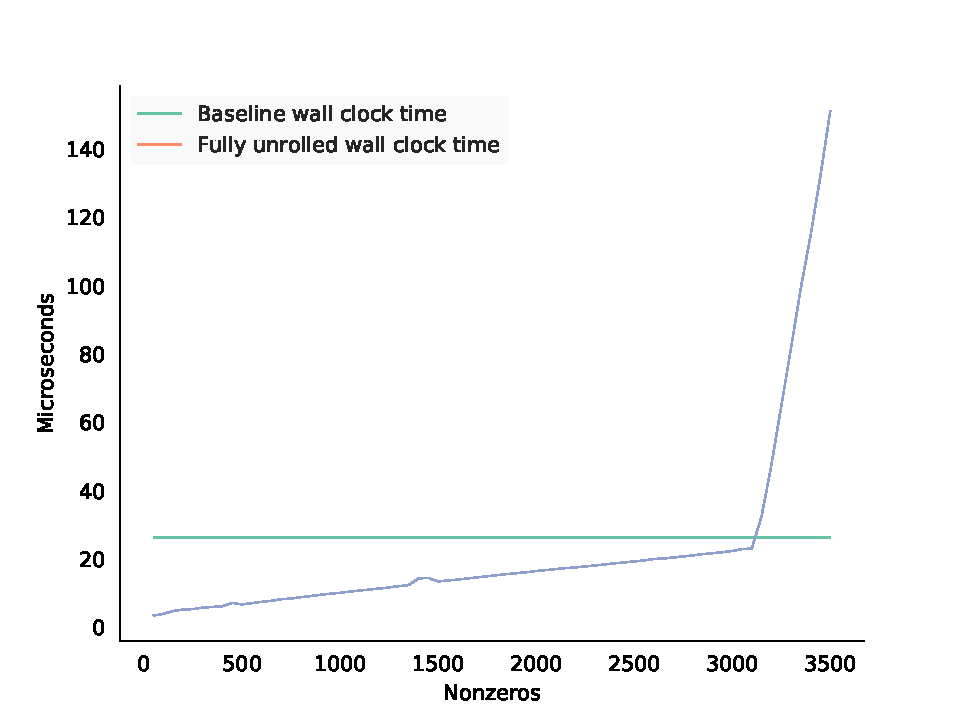
\includegraphics[width=\textwidth]{images/fig2.pdf}
      \caption{Time to solution for unrolledsparse}
      \label{fig:unrolled_time}
    \end{subfigure}
    \begin{subfigure}[b]{0.4\textwidth}
      \centering
      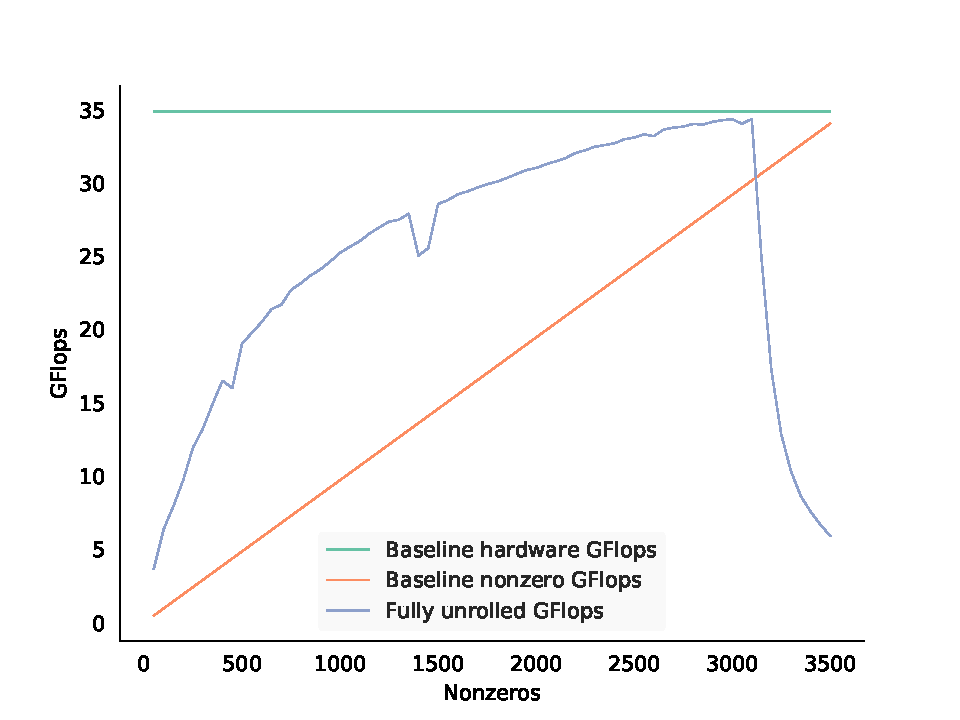
\includegraphics[width=\textwidth]{images/fig3.pdf}
      \caption{Performance of unrolledsparse}
      \label{fig:unrolled_perf}
    \end{subfigure}
  \end{figure}

  \begin{itemize}
    \item For $nnz < 3100$, time-to-solution scales linearly.
    \item For $nnz > 3200$, the FMAs completely fill the instruction cache (regardless of matrix dimensions!)
    \item Fully unrolled sparse algorithm outperforms dense ``nonzero'' GFlops, but always underperforms dense ``hardware'' GFlops
    
  \end{itemize}


\section{Performance of general dense-by-sparse multiplication}

\section{Performance of SeisSol proxy}

\section{Performance of tensor multiplication}